\documentclass[landscape]{article}
%ss[10pt,landscape]{article}
\usepackage{multicol}
\usepackage{calc}
\usepackage{ifthen}
\usepackage[landscape]{geometry}
\usepackage{amsmath,amsthm,amsfonts,amssymb}
\usepackage{color,graphicx,overpic}
\usepackage{wrapfig}
\usepackage{hyperref}
\usepackage[shortlabels]{enumitem}
\usepackage{enumerate}



\pdfinfo{
/Title (170_cheat_sheet.pdf)
/Creator (TeX)
/Producer (pdfTeX 1.40.0)
/Author (Nate Holland)
/Subject (CS170)
/Keywords (pdflatex, latex,pdftex,tex)}

% This sets page margins to .5 inch if using letter paper, and to 1cm
% if using A4 paper. (This probably isn't strictly necessary.)
% If using another size paper, use default 1cm margins.
\ifthenelse{\lengthtest { \paperwidth = 11in}}
    { \geometry{top=.3in,left=.3in,right=.3in,bottom=.3in} }
    {\ifthenelse{ \lengthtest{ \paperwidth = 297mm}}
        {\geometry{top=1cm,left=1cm,right=1cm,bottom=1cm} }
        {\geometry{top=1cm,left=1cm,right=1cm,bottom=1cm} }
    }

% Turn off header and footer
\pagestyle{empty}

% Redefine section commands to use less space
\makeatletter
\renewcommand{\section}{\@startsection{section}{1}{0mm}%
                            {-1ex plus -.5ex minus -.2ex}%
                            {0.5ex plus .2ex}%x
                            {\normalfont\large\bfseries}}
\renewcommand{\subsection}{\@startsection{subsection}{2}{0mm}%
                            {-1explus -.5ex minus -.2ex}%
                            {0.5ex plus .2ex}%
                            {\normalfont\normalsize\bfseries}}
\renewcommand{\subsubsection}{\@startsection{subsubsection}{3}{0mm}%
                            {-1ex plus -.5ex minus -.2ex}%
                            {1ex plus .2ex}%
                            {\normalfont\small\bfseries}}
\makeatother

% Define BibTeX command
\def\BibTeX{{\rm B\kern-.05em{\sc i\kern-.025em b}\kern-.08em
    T\kern-.1667em\lower.7ex\hbox{E}\kern-.125emX}}

% Don't print section numbers
\setcounter{secnumdepth}{0}


\setlength{\parindent}{0pt}
\setlength{\parskip}{0pt plus 0.5ex}

%My Environments
\newtheorem{example}[section]{Example}
% -----------------------------------------------------------------------

\def\ci{\perp\!\!\!\perp}



\begin{document}
\raggedright
\footnotesize
\begin{multicols}{3}


% multicol parameters
% These lengths are set only within the two main columns
%\setlength{\columnseprule}{0.25pt}
\setlength{\premulticols}{1pt}
\setlength{\postmulticols}{1pt}
\setlength{\multicolsep}{1pt}
\setlength{\columnsep}{2pt}

\begin{center}
    \Large{\underline{CS 170 Cheat Sheet}} \\
\end{center}

\subsection*{Big O notation}

$ f, g \in \mathbb{N}$, $f = O(g)$ means that f grows no faster than g if $\exists c > 0$ s.t. $F(n) \leq c g(n)$ 

$ f = \Theta(g)$ means $g = O(f)$

$f = \Theta(g)$ IFF $ f = O(g) \ \& \ g = \Theta(g)$


\subsection*{Master Theorem}
Given: $T(n) = a \times T(\frac{n}{b}) + O(n^d)$

\begin{description}

\item[a)]
$O(n^d)$ if $d > log_b(a)$

\item[b)]
$O(n^dlog(n))$ if $d = log_b(a)$

\item[c)]
$O(n^{log_b(a)})$ if $d < log_b(a)$

\end{description}

\subsection*{Graph Algorithms}

\textbf{DFS: O(V + E)}

Guaranteed to visit every node reachable by $v$ before returning from $v$.
Can create topological sort of DAG.

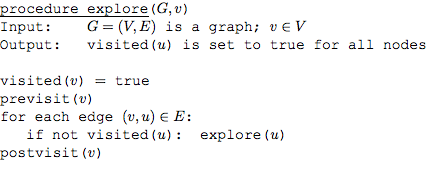
\includegraphics[scale=0.5]{DFS}

\textbf{BFS: O(V + E)}

Used to find shortest path through an unweighted graph.

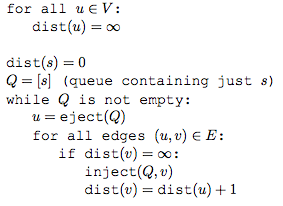
\includegraphics[scale=0.5]{BFS}

\textbf{Dijkstras: O((V + E) log V)}

Like BFS but with priority queue, used to find shortest path between two nodes on a weighted graph.

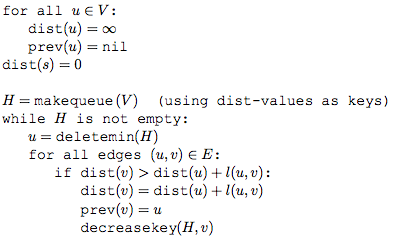
\includegraphics[scale=0.5]{dijkstra}

\textbf{Bellman Ford: O((V  E)}

Find shortest paths with negative edges as long as there are no negative cycles. Runs $V -1$ updates on all E edges.

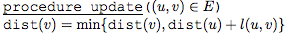
\includegraphics[scale=0.5]{BF1}

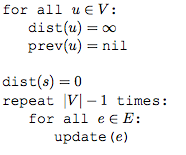
\includegraphics[scale=0.5]{BF2}

\textbf{Floyd-Warshall: $O((V^3)$}

Find the shortest path between all pairs of vertexes in a graph.

\textbf{Kruskal: O((E log(V))}

Use the disjoint set trees to add edges in ascending order that don't complete a cycle. Used to find MST.

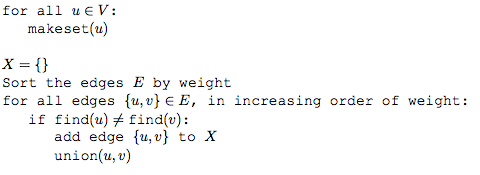
\includegraphics[scale=0.5]{kruskal}

\textbf{Prim's: O((E log(V))}

On each iteration, the subtree defined by X grows by one edge, namely, the lightest edge
between a vertex in S and a vertex outside S

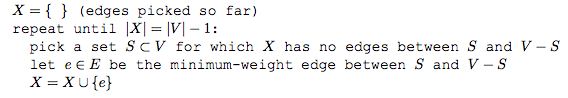
\includegraphics[scale=0.42]{prim}

\textbf{Cut Property:}
Suppose edges $X$ are part of a minimum spanning tree of
$G = (V, E)$. Pick any subset of nodes $S$ for which $X$ does not
cross between $S$ and $V-S$, and let $e$ be the lightest edge across the
partition. Then $X \cup e$ is part of some Minimum Spanning Tree.



\textbf{Huffman Encoding O(n log n) }

Make a tree of decisions of whether to pick a 0 or a 1, make all the leaves values.
Then we can follow the tree down to decode a Huffman encoding of values.

\subsection{FFT}

It is a black box which represents 2 polynomials as a list of points and then multiplies them together to create a new polynomial. Takes \textbf{O(N log N)} time. Uses roots of unity to determine where to multiply two polynomials together.

\textbf{$N^{th}$ Roots of Unity} can be found by: $ cos(\frac{2\pi j}{n}) + i \cdot sin(\frac{2\pi j}{n})$


\subsection{Dynamic Programming}

These are normally straight forward, mainly we just need to find a recursive relationship for sub problems and then figure out the order in which we need to solve them.
Normally runtime can easily be deduced by the number of for loops we have to run to.
Following are some basic examples of dynamic programming in case we see something like these on the final.

\textbf{Edit Distance: $O(n^2)$}

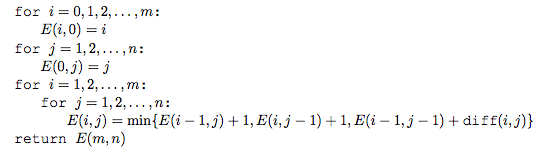
\includegraphics[scale=0.42]{edit}

\textbf{Knapsack with repetition: $O(nW)$}

K(w) is the maximum value we can achieve with weight w.

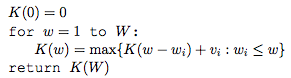
\includegraphics[scale=0.5]{knapNR}

\textbf{Knapsack without repetition: $O(nW)$}

$K(w, j)$ = maximum value achievable using a knapsack of capacity $w$ and items $1, . . . , j$.

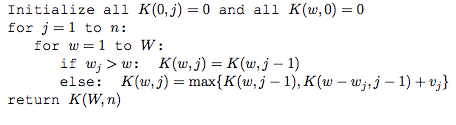
\includegraphics[scale=0.5]{knapWR}

\subsection{Linear Programming}

Linear Programming is a way to state problems as systems of equations and then we can solve them in polynomial time as long as we don't need Integer Linear Programming, which is NP Complete.
It can be solved with the simplex method which we don't need to know, can just treat it like a black box.

\textbf{Remember:} when writing out your solutions make sure you add the non-negative constraints.

\subsection{Max Flow}

This is bounded by $O( C \cdot E)$ or $O ( V \cdot E^2)$

\textbf{Max-flow min-cut theorem:} the size of the maximum flow in a network equals the capacity of the smallest (s,t) cut.

\textbf{Maximum flow property:} if all edge capacities are integers, then the optimal flow found by our algorithm is integral. We can see this directly from the algorithm, which in such cases would increment the flow by an integer amount on each iteration.

When drawing the residuals make sure you draw the flow you've already used backwards, so some paths with have an arror going forward and an arror going backward.

\newpage 
\subsection{P/NP}

\textbf{P:} search problem that can be solved in polynomial time.

\textbf{NP:} search problem that can be checked to be correct in polynomial time.

\textbf{NP complete:} search problem that is at least as hard as every other NP complete problem. Basically it reduces to circuit sat, could possibly be solved in polynomial time but we doubt it.

\textbf{NP hard:} there exists NP complete Y such that Y is reducible to X but can't go the other way around. Not actually in NP.

Here are some examples of \textbf{P} and \textbf{NP} algorithms:

\begin{tabular}{| l | l |}
  \hline
  \textbf{NP} & \textbf{P} \\ \hline
  3+ SAT & 2 SAT \\ \hline
  TSP & MST \\ \hline
  Longest Path & Shortest Path \\ \hline
  3D Matching & Bipartide matching \\ \hline
  Knapsack & Unary Knapsack \\ \hline
  Independent Set & Independent Set on Trees \\ \hline
  Integer LP & Linear Programming \\ \hline
  Rudrata Path & Euler Path \\ \hline
  Balanced Cut & Minimum cut \\ \hline
\end{tabular}




\subsection{Reductions}
A search problem is NP-complete if all other search problems reduce to it.

Make sure that the conversions between the two algorithms are of polynomial size and time, otherwise the reduction does not work.

To reduce X to Y means to find a solution for X using Y.

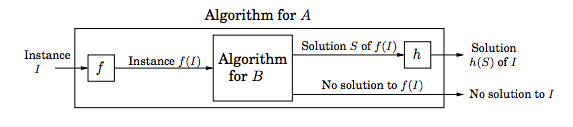
\includegraphics[scale=0.42]{reduction}









\rule{0.3\linewidth}{0.25pt}
\newpage
\scriptsize
\bibliographystyle{abstract}
\bibliography{refFile}
\end{multicols}
\end{document}